\documentclass[a4paper,12pt]{article} % тип документа

\newcommand\nameone{Цыганкова Екатерина}
\newcommand\groupone{Б02-409}
\newcommand\labnumber{4.7.3}
\newcommand\labwork{Поляризация}
%%% Работа с русским языком
\usepackage{cmap}					% поиск в PDF
\usepackage{mathtext} 				% русские буквы в формулах
\usepackage[T2A]{fontenc}			% кодировка
\usepackage[utf8]{inputenc}			% кодировка исходного текста
\usepackage[main = russian, english]{babel}	% локализация и переносы
%\selectlanguage{english} (для англостатей)
%\usepackage{caption}

%%% Дополнительная работа с математикой
\usepackage{amsmath,amsfonts,amssymb,amsthm,mathtools} % AMS
\usepackage{icomma}
\usepackage{physics}
\usepackage{multicol}
\usepackage{bm}
\usepackage{mathrsfs}
\usepackage{verbatim}

%%% Номера формул
%\mathtoolsset{showonlyrefs=true} 
%\usepackage{leqno} 

%%% Свои команды
\DeclareMathOperator{\sgn}{sgn}

\usepackage{csquotes} 
\usepackage[backend=biber,style=authoryear]{biblatex}


%%% Работа с графикой
\usepackage{graphicx}
\graphicspath{{images/}}  
\setlength\fboxsep{3pt} 
\setlength\fboxrule{1pt} 
\usepackage{wrapfig} 
\usepackage{subcaption}
\usepackage{tikz}
\usepackage{pgfplots}
\usepackage{pgfplotstable}
\usepgfplotslibrary{polar}
\pgfplotsset{compat=1.18} 

%%% Работа с таблицами
\usepackage{array,tabularx,tabulary,booktabs}
\usepackage{longtable}  
\usepackage{multirow} 
\usepackage{soul} 

%%% Теоремы
\theoremstyle{plain} 
\newtheorem{theorem}{Th}[section]
\newtheorem{proposition}[theorem]{Proposition}
\newtheorem{question}{Question}[section]
 
\theoremstyle{definition} 
\newtheorem{corollary}{Corollary}[theorem]
\newtheorem{problem}{Problem}[section]
\newtheorem{definition}{Def}[section]
 
\theoremstyle{remark} 
\newtheorem*{nonum}{Solution}

%%% Программирование
\usepackage{etoolbox} 

%%% Гиперссылки
\usepackage{hyperref}

\usetikzlibrary{knots}
\usepackage{tcolorbox}

%%% Страница
\usepackage{geometry} 
	\geometry{top=20mm, bottom=20mm, left=15mm, right=20mm}

\usepackage{setspace} 

\usepackage{lastpage} 
\usepackage{amssymb}
\usepackage{xcolor}
\usepackage[all]{xy}
\usepackage{dsfont}



\begin{document}
\begin{center}   
	\large{Лабораторная работа № \labnumber\\ \hfill \break\Large{\textbf{\labwork}}}\\
    \normalsize
    \begin{flushright}
    \nameone, \groupone \\
    \today
    \end{flushright}
\end{center}
\begin{center}
    В работе изучаются свойства поляризованного света, способы его получения и оптические элементы для его анализа: поляризаторы и двоякопреломляющие пластины. Предложены методы определения главных направлений поляризатора и двоякопреломляющей пластины. Изучена поляризация преломленного и отраженного света, а также интерференция поляризованного света.
\end{center}

\tableofcontents

\newpage

\section{Теоретическое введение}
\subsection{Поляризация отраженного и преломленного света}
\begin{figure}[h]
    \centering
    \begin{subfigure}{0.48\textwidth}
        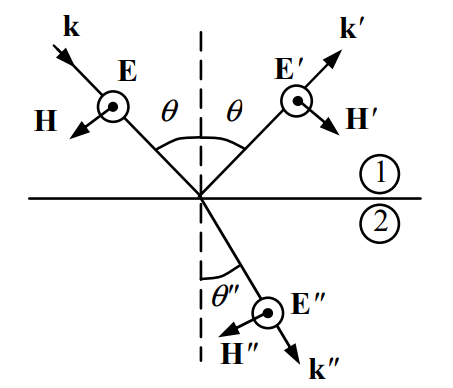
\includegraphics[width = 0.9\textwidth]{pics/fren_s}
        \caption{s-поляризация}
    \end{subfigure}
    \hfill
    \begin{subfigure}{0.48\textwidth}
        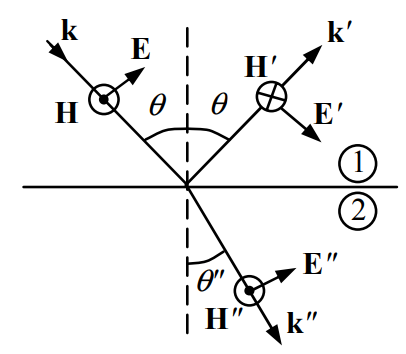
\includegraphics[width = 0.9\textwidth]{pics/fren_p}
        \caption{p-поляризация}
    \end{subfigure}
    \caption{}
    \label{fig:fren}
\end{figure}

Коэффициенты отражения  ($r \equiv \frac{E'}{E}$) и преломления ($t \equiv \frac{E''}{E}$) для s- ($\perp$) и p- ($\parallel$) поляризаций (см Рис. \ref{fig:fren}) определяются по формулам Френеля:

\begin{equation}
    \label{eq:fren}
\begin{aligned}
    r_\perp &= -\frac{\sin(\theta - \theta'')}{\sin(\theta + \theta'')}  &t_\perp &= \frac{2 \cos\theta \sin\theta''}{\sin(\theta + \theta'')} \\
    r_\parallel &= \frac{\tg(\theta - \theta'')}{\tg(\theta + \theta'')}  &t_\parallel &= \frac{2 \cos \theta \sin\theta''}{\sin(\theta + \theta'')\cos(\theta - \theta'')}
\end{aligned}
\end{equation}

, а $\theta$ и $\theta''$ связаны законом Снеллиуса: $\sin\theta = n\sin\theta''$ ($n_1 = 1$, $n_2 = n$).

Из приведенных формул \eqref{eq:fren} видно, что при $\theta + \theta'' = \frac{\pi}{2}$ коэффициент отражения для p-поляризованного света равен нулю. Соотвествующий угол падения $\tan \theta_\text{бр} = n$ называется углом Брюстера. 

Таким образом, если на плоско-параллельную пластинку под углом Брюстера падает неполяризованный свет, то отраженный свет имеет линейную s-поляризацию, а для проходящего света отношение интенсивностей s- и p-поляризаци, согласно \eqref{eq:fren}, определяется как:

\begin{equation}
    \label{eq:trans_polar}
    \frac{T_\perp}{T_\parallel} = \sin^4 2\alpha_\text{бр}
\end{equation}

\subsection{Двоякопреломляющие пластинки и интерференция поляризованного света}

Двоякопреломляющая пластинка
имеет два взаимно перпендикулярных
главных направления. Волны, поляризованные
вдоль главных направлений, распространяются в пластинке с разными
скоростями, не изменяя характера своей
поляризации.

В работе изучаются двоякопреломляющие пластинки трех типов: $\frac{\lambda}{4}$, $\frac{\lambda}{2}$ и $\lambda$. 

\subsubsection{Изменение поляризации линейно-поляризованного света при прохождении пластин}
\label{subsec:polar_lam}

\begin{wrapfigure}{r}{0.3\textwidth}
    \begin{center}
    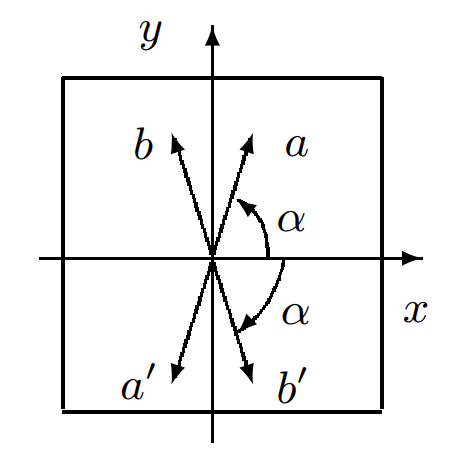
\includegraphics[width = 0.28\textwidth]{pics/lam2_rot}
    \caption{Поворот направления колебаний после прохождения пластинки $\frac{\lambda}{2}$}
    \label{fig:lam2_rot}
    \end{center}
\end{wrapfigure}

\textbf{1) $\bm{\lambda}$.} Поляризация не изменяется.

  \textbf{2) $\bm{\frac{\lambda}{2}}$.} Направление поляризации испытавает отражение относительно главных осей пластины (смю Рис. \ref{fig:lam2_rot}).

  \textbf{3) $\bm{\frac{\lambda}{4}}$.} Возникает эллиптическая поляризация. Оси эллипса совпадают с главными осями пластины. Если направление колебаний, падающего на пластину света, составляет угол $45^\circ$ с главными осями пластины, то итоговая поляризация оказывается круговой.

\subsubsection{Пластинка чувствительного оттенка}
\label{subsec:color_pl}
Для определения <<быстрой>> и <<медленной>> осей пластинки $\frac{\lambda}{4}$ в работе используется пластинка чувствительного оттенка $\lambda$ для зеленого цвета. Пластинка имеет форму стрелы (см. Рис. \ref{fig:color_pl}), вдоль оси которой расположено главное направление, соответствующее большей скорости распространения. 

\begin{wrapfigure}{l}{0.2\textwidth}
    \begin{center}
    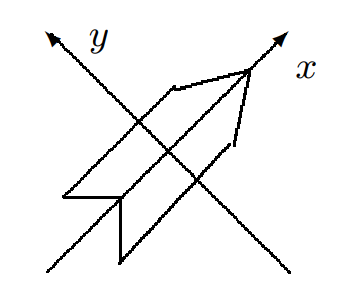
\includegraphics[width = 0.18\textwidth]{pics/color_pl}
    \caption{Пластинка чувствительного оттенка}
    \label{fig:color_pl}
    \end{center}
\end{wrapfigure}

Если установить пластинку чувствительного оттенка под некоторым углом между двух скрещенных поляроидов, то зеленая компонента света, будет задержана вторым поляроидом, в то время как компоненты других длин волн, поляризация которых изменится после прохождения пластинки, частично пройдут через систему. Поэтому пластинка будет казаться окрашенной в лилово-красный цвет.

Если добавить к пластинке чувствительного оттенка пластинку $\frac{\lambda}{4}$ так, чтобы направления их <<быстрых>> осей совпадали, мы получим пластинку $\lambda$ уже для красного цвета. Поэтому выходящий свет будет бирюзовым.

Если, наконец, добавить к пластинке чувствительного оттенка пластинку $\frac{\lambda}{4}$ так, чтобы направление <<быстрой>> оси первой совпадало с направлением <<медленной>> оси второй, мы получим пластинку $\lambda$ для фиолетового цвета цвета. Поэтому выходящий свет будет оранжево-желтым.

\subsubsection{Интерференция поляризованного света}
\label{subsec:polariz}
\begin{wrapfigure}{r}{0.3\textwidth}
    \begin{center}
    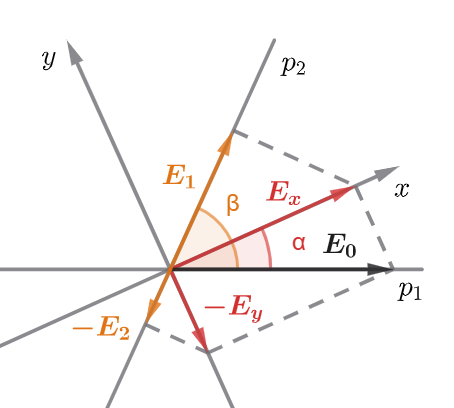
\includegraphics[width = 0.28\textwidth]{pics/polariz}
    \caption{Интерференция поляризованных лучей}
    \label{fig:color_pl}
    \end{center}
\end{wrapfigure}
Рассмотрим двоякопреломляющую пластину между двух поляроидов. В данном пункте обсуждается, как яркость и цвет выходящего света зависят от угла между поляроидами $\beta$ и угла между первым поляроидом и <<быстрой>> осью пластины $\alpha$.

Рассмотрим два частных случая.

\textbf{Скрещенные поляризаторы ($\bm{\beta = 90^\circ}$); переменный $\bm{\alpha}$.}

В этом случае $E_2 = -E_1 = E_0 \sin\alpha \cos\alpha$. Следовательно, для пластинки, дающей набег фазы $\Delta\phi(\lambda)$ по оси x, результирующая интенсивность оказывается:

\begin{equation}
    I = 2E_0^2 \cos^2\alpha \sin^2\alpha (1 - \cos\Delta\phi(\lambda))
\end{equation}

Отсюда видно, что при изменении угла $\alpha$ интенсивность для всех длин волн изменяется пропорционально. Поэтому при вращении пластины между скрещенных поляроидов изменяется только интенсивность выходящего света, но не его цвет.

\textbf{$\bm{\alpha = 45^\circ}$ -- фиксирован; переменный $\bm{\beta}$.}


В этом случае $E_1 = \frac{E_0}{2}(\sin\beta + \cos\beta)$, $-E_2 = \frac{E_0}{2}(\sin\beta - \cos\beta)$. Следовательно, для пластинки, дающей набег фазы $\Delta\phi(\lambda)$ по оси x, результирующая интенсивность оказывается:

\begin{equation}
    I = \frac{E_0^2}{2}(1 + \cos(2\beta)\cos\Delta\phi(\lambda))
\end{equation}

Видно, что когда $\beta = 45^\circ$, то есть когда разрешенное направление второго поляризатора совпадает с главной осью пластины, различия в интенсивности между светом разных длин волн пропадает.

Также, можно заметить, что если для света некоторой длины волны при $\beta = 0^\circ$ достигалась максимальная интенсивность, то при повороте второго поляризатора на $\beta = 90^\circ$, интенсивность света этой же длины волны оказывается минимальной. Поэтому в случаях параллельных и скрещенных поляризаций поляроидов пластинка приобретает <<дополнительные>> друг к другу цвета.

\subsubsection{Определение направления вращения элиптически поляризованного света}

Для анализа эллиптически поляризованного света в работе используется пластинка $\frac{\lambda}{4}$. Если разместить ее так, чтобы главная ось поляризациии света $ox$ совпадала с <<быстрой>> главной осью пластинки, то на выходе получится линейно поляризованный свет. По направлению поляризации можно тогда определить, в какую сторону был закручен вектор напряженности исследуемого эллиптически-поляризованного света (см. Рис. \ref{fig:ellipt_polar}).

\begin{figure}[h]
  \centering
    \caption{Изменение поляризации света после прохождения пластинки $\frac{\lambda}{4}$ с быстрой осью $ox$}
    \label{fig:ellipt_polar}
  \begin{subfigure}[t]{\textwidth}
    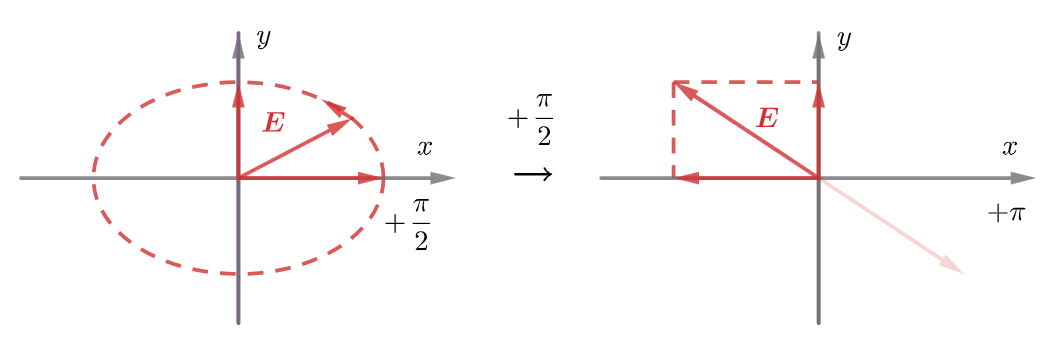
\includegraphics[width=0.9\textwidth]{pics/8_anti_clockwise}
  \end{subfigure}
\begin{subfigure}[t]{\textwidth}
    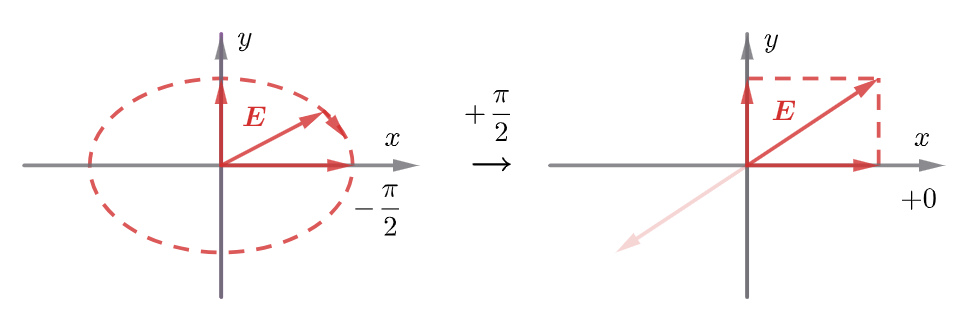
\includegraphics[width=0.9\textwidth]{pics/8_clockwise}
  \end{subfigure}
\end{figure}

\clearpage

\section{Изучение поляризации отраженного и преломленного света}
\textbf{\textcolor{red}{Все пункты работы проводились на установке №7}}

\subsection{Определение разрешенных направлений поляроидов}

Для определения разрешенных направлений поляроида можно использовать схему, изображенную на Рис. \ref{fig:setup_1}. Минимум интенсивности отраженного света тогда наблюдается при падении света на черное зеркало под углом Брюстера и горизонтальном разрешенном направлении поляроида (см. Рис. \ref{fig:1_bm_min} и \ref{fig:1_bm_simp}).
\begin{figure}[h]
    \centering
  \begin{subfigure}[t]{0.45\textwidth}
    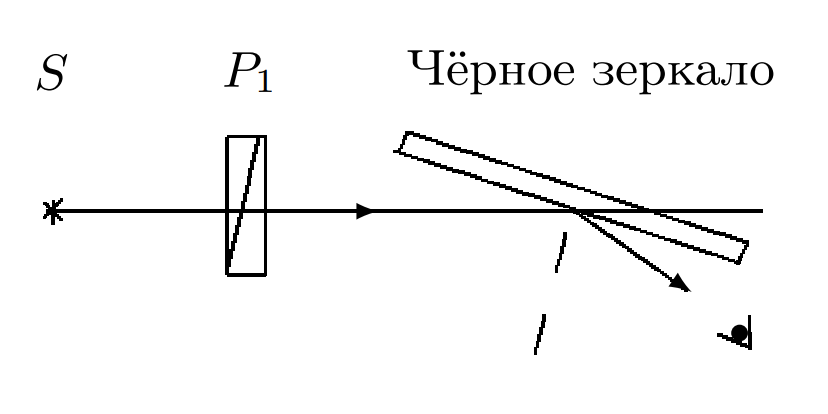
\includegraphics[width=0.9\textwidth]{pics/setup_1}
    \caption{Схема установки (вид сверху)}
    \label{fig:setup_1}
  \end{subfigure}
  \hfill
  \begin{subfigure}[t]{0.25\textwidth}
    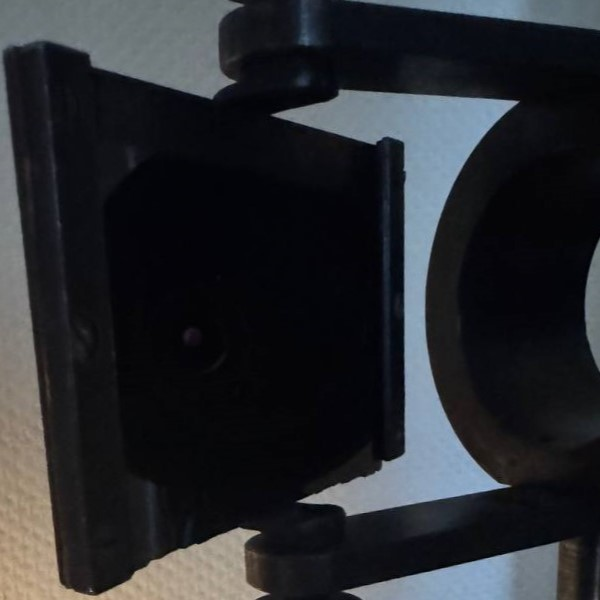
\includegraphics[width=0.9\textwidth]{exp_pics/1_1_black_mirror_min}
    \caption{Отраженный от черного зеркала свет при падении под углом брюстера и горизонтальном разрешенном направлении поляроида}
    \label{fig:1_bm_min}
  \end{subfigure}
  \hfill
  \begin{subfigure}[t]{0.25\textwidth}
    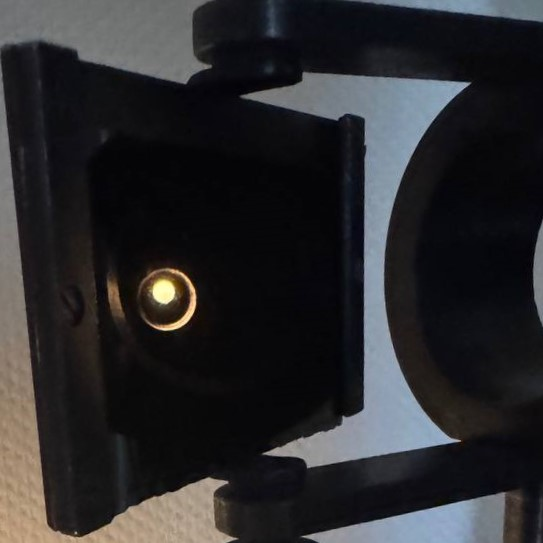
\includegraphics[width=0.9\textwidth]{exp_pics/1_1_black_mirror_simp}
    \caption{Отраженный от черного зеркала свет при других углах падения}
    \label{fig:1_bm_simp}
  \end{subfigure}
  \caption{Определение разрешенного направления поляроида с помощью черного зеркала}
\end{figure}

Когда разрешенное направление одного из поляроидов определено с использованием черного зеркала, для определения разрешенного направления второго поляроида можно воспользоваться схемой \ref{fig:setup_1_2}. Минимум интенсивности проходящего света тогда наблюдается при скрещенных (расположенных под $90^\circ$) разрешенных направлениях поляроидов (см. Рис. \ref{fig:1_polar_0} и \ref{fig:1_polar_90}). 

\begin{figure}[h]
    \centering
  \begin{subfigure}[t]{0.45\textwidth}
    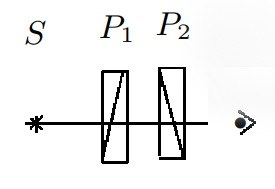
\includegraphics[width=0.8\textwidth]{pics/setup_1_2}
    \caption{Схема установки}
    \label{fig:setup_1_2}
  \end{subfigure}
  \hfill
\begin{subfigure}[t]{0.25\textwidth}
    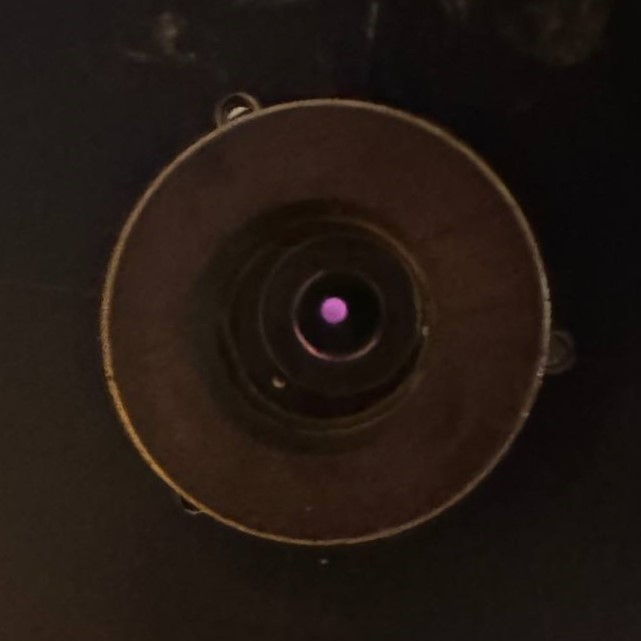
\includegraphics[width=0.8\textwidth]{exp_pics/1_2_polar_90}
    \caption{Проходящий через поляроиды свет при скрещенных разрешенных направлениях}
    \label{fig:1_polar_90}
  \end{subfigure}
  \hfill
  \begin{subfigure}[t]{0.25\textwidth}
    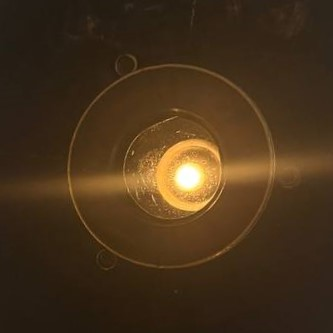
\includegraphics[width=0.8\textwidth]{exp_pics/1_2_polar_0}
    \caption{Проходящий через поляроиды свет при параллельных разрешенных направлениях}
    \label{fig:1_polar_0}
  \end{subfigure}
  \caption{Определение разрешенного направления поляроида с помощью поляроида с известным разрешенным направлением}
\end{figure}
\newpage
\subsection{Определение показателя преломления эбонита по углу Брюстера}
\label{subsec:ebon}

После замены в схеме \ref{fig:setup_1} черного зеркала на эбонитовую пластину и установки разрешенного направления поляроида по горизонтали, по минимуму интенсивности отраженного света (см. Рис. \ref{fig:2}) был определен угол Брюстера для эбонита $\theta_\text{бр} = (57 \pm 3)^\circ$. 

Отсюда коэффициент преломления эбонита $\boxed{n_\text{эксп} = \tg \theta_\text{бр} = 1,54 \pm 0,18}$. \ul{олученный результат в пределах погрешности совпадает с табличным $n_\text{табл} = 1,6 \divisionsymbol 1,7$}.

\begin{figure}[h]
    \centering
    \begin{subfigure}[t]{0.3\textwidth}
    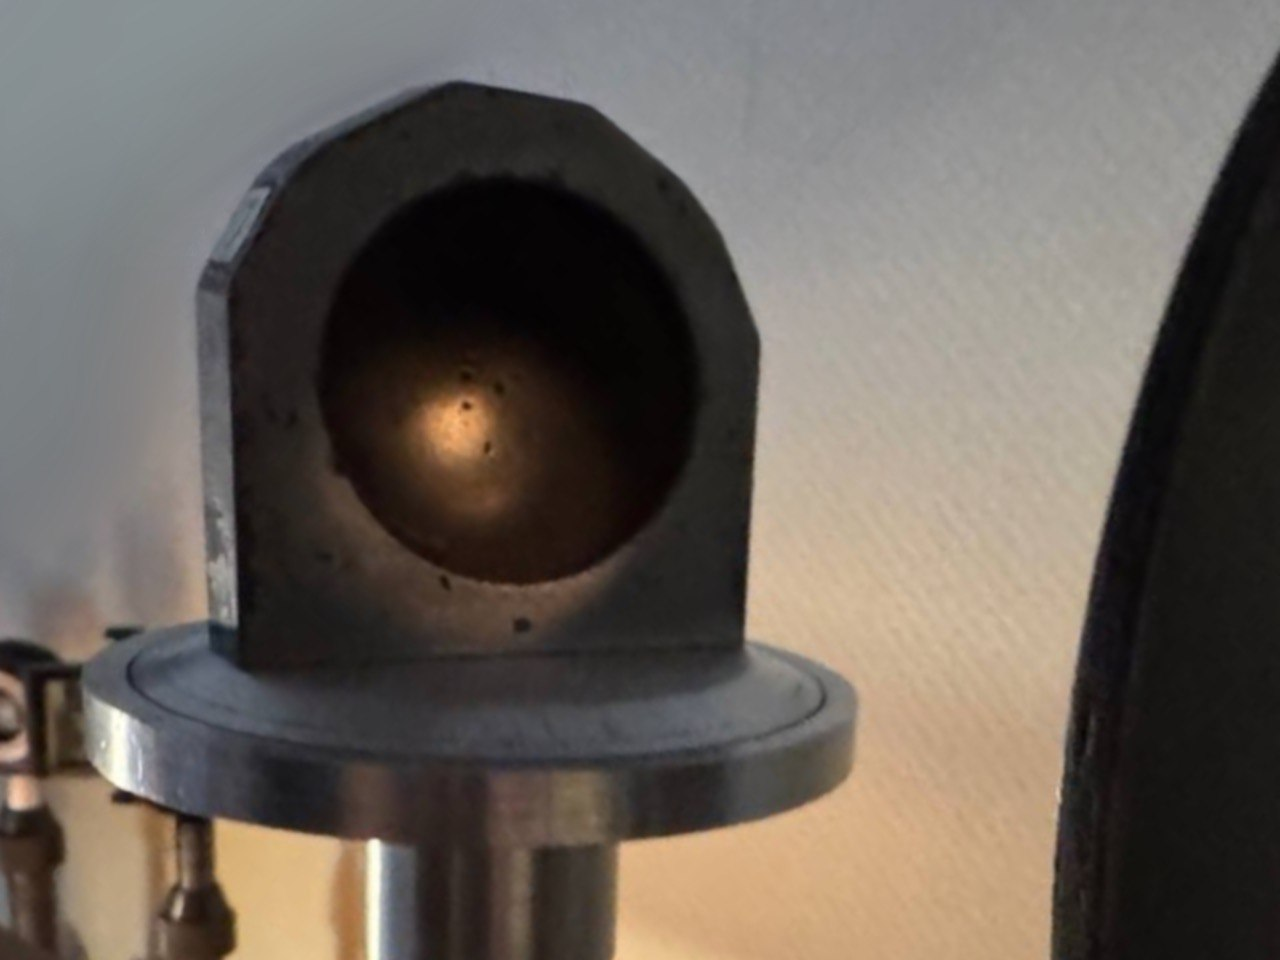
\includegraphics[width=0.9\textwidth]{exp_pics/2_little_ang}
    \caption{$\theta < \theta_\text{бр}$}
  \end{subfigure}
  \hfill
  \begin{subfigure}[t]{0.3\textwidth}
    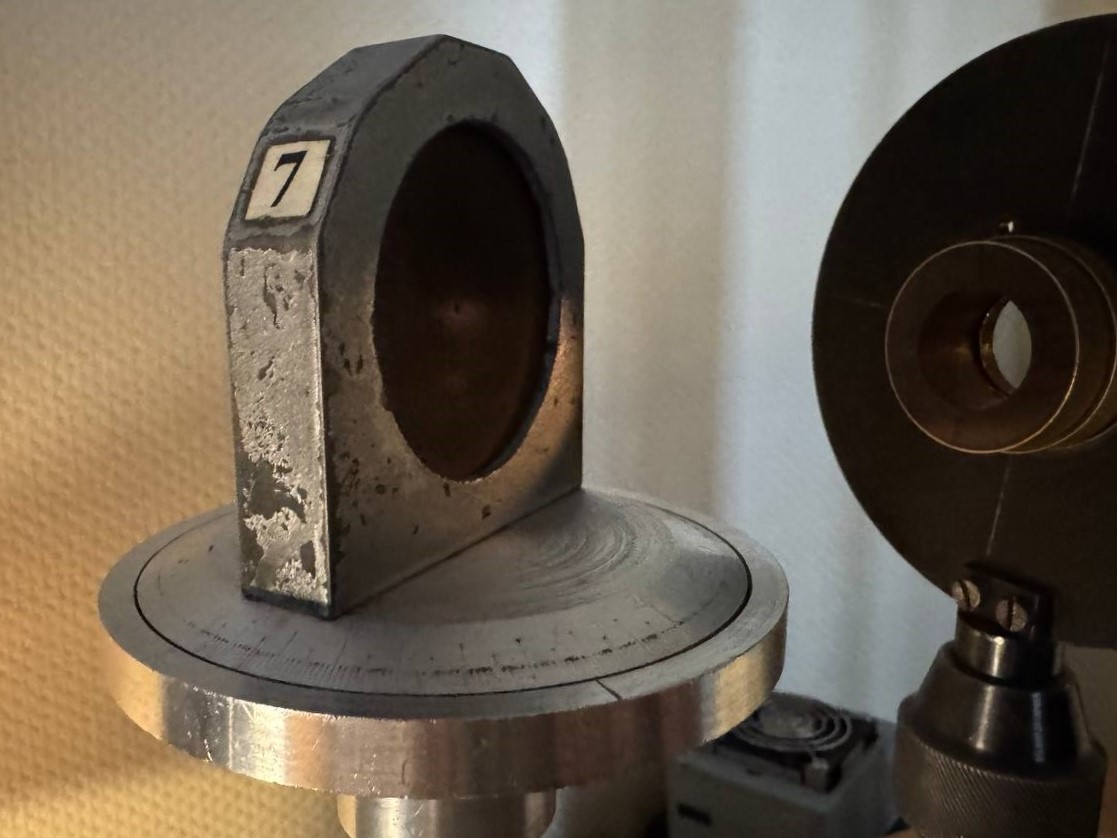
\includegraphics[width=0.9\textwidth]{exp_pics/2_bruster_ang}
    \caption{$\theta = \theta_\text{бр}$}
  \end{subfigure}
  \hfill
  \begin{subfigure}[t]{0.3\textwidth}
    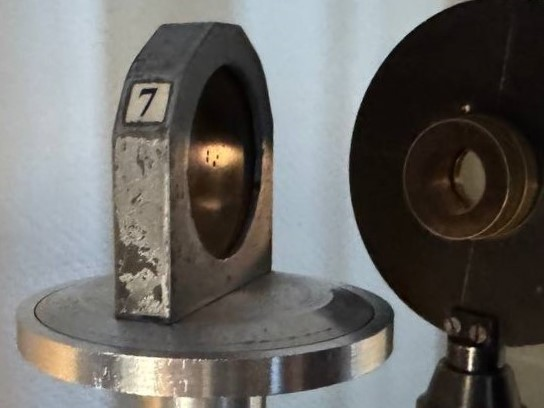
\includegraphics[width=0.9\textwidth]{exp_pics/2_great_ang}
    \caption{$\theta > \theta_\text{бр}$}
  \end{subfigure}
  \caption{Интенсивность отраженного от эбонитовой пластины света при разных углах падения $\theta$}
  \label{fig:2}
\end{figure}
\subsection{Наблюдение поляризации отраженного и преломленного света}

\begin{figure}[h]
    \centering
    \caption{Изучение поляризации отраженного и преломленного света}
    \begin{subfigure}[t]{0.4\textwidth}
    \caption{Cхема установки (вид сверху). \\
    Ф -- зеленый светофильтр}
    \label{fig:setup_3}
    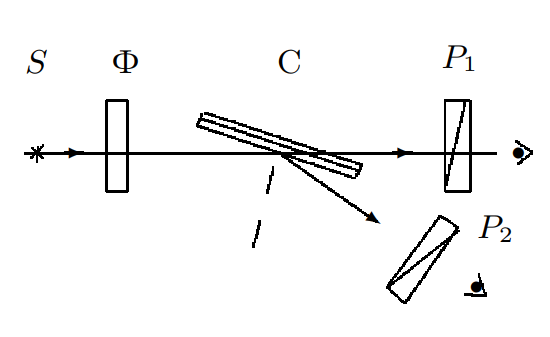
\includegraphics[width=0.9\textwidth]{pics/setup_3}
  \end{subfigure}
  \hfill
  \begin{subfigure}[t]{0.28\textwidth}
    \caption{Интенсивность отраженного света, поляризованного по ...}
    \label{fig:3_refl}
    \centering
    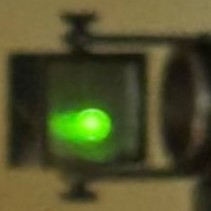
\includegraphics[width=0.9\textwidth]{exp_pics/3_2_refl_vert_polar}\\
    ... вертикали\\
    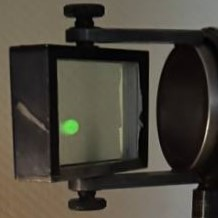
\includegraphics[width=0.9\textwidth]{exp_pics/3_2_refl_hor_polar}\\
    ... горизонтали\\
  \end{subfigure}
  \hfill
  \begin{subfigure}[t]{0.28\textwidth}
    \caption{Интенсивность преломленного света, поляризованного по ...}
    \label{fig:3_refr}
    \centering
    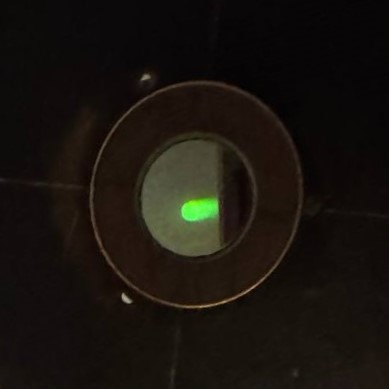
\includegraphics[width=0.9\textwidth]{exp_pics/3_3_refr_vert_polar}\\
    ... вертикали\\
    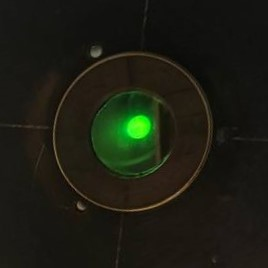
\includegraphics[width=0.9\textwidth]{exp_pics/3_3_refr_hor_polar}\\
    ... горизонтали\\
  \end{subfigure}
\end{figure}

\begin{wrapfigure}{r}{0.25\textwidth}
    \begin{center}
    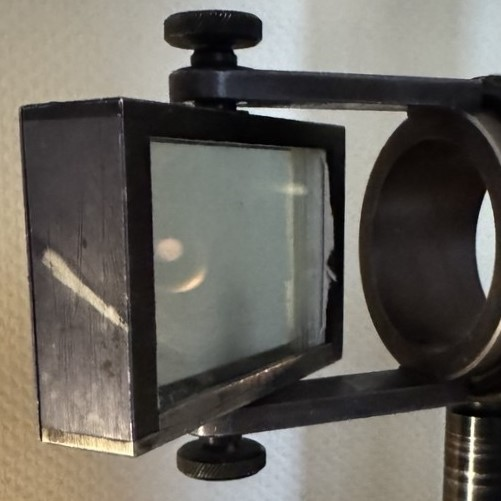
\includegraphics[width = 0.23\textwidth]{exp_pics/3_1_bruster_ang}
    \caption{Отраженный p-поляризованный свет при падении на стопу стеклянных пластин под углом Брюстера}
    \label{fig:3_brust}
    \end{center}
\end{wrapfigure}

В данном пункте работы изучалась поляризация отраженного и преломленного света в стопе стеклянных пластин. Изначально, используя схему \ref{fig:setup_1} с исследуемой стопой пластин вместо черного зеркала, было выбрано ее направление, соответствующее падению света под углом Брюстера (см. Рис. \ref{fig:3_brust}). Далее, не меняя направления пластинок, по схеме \ref{fig:setup_3} наблюдался характер поляризации отраженного и преломленного света.

Как видно из Рис. \ref{fig:3_refl}, при падении под углом Брюстера отраженный свет поляризован по вертикали. Для преломленного же света (см. Рис. \ref{fig:3_refr}), в согласии с \ref{eq:trans_polar}, интенсивность горизонтально поляризованной составляющей выше, чем вертикально поляризованной.

\section{Изучение двоякопреломляющих пластинок и эллиптически поляризованного света}
\subsection{Определение главных осей двоякопреломляющих пластинок}

\begin{wrapfigure}{r}{0.3\textwidth}
    \begin{center}
    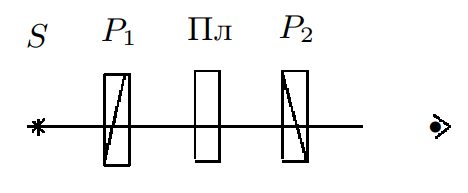
\includegraphics[width = 0.28\textwidth]{pics/setup_4}
    \caption{Определение главных осей пластинок}
    \label{fig:setup_4}
    \end{center}
\end{wrapfigure}

Для определения главных осей двоякопреломляющих пластинок, была использована схема \ref{fig:setup_4}. Вращением исследуемой пластинки, установленной между скрещенных поляроидов, мы добивались минимума интенсивности проходящего света, что соответствует совпадению главных осей пластинки с разрешенными направлениями поляроидов. По результатам измерений были получены следующие главные направления для первой и второй пластинок:

\begin{equation}
    \begin{aligned}
    1: ~~~ 58^\circ &\leftrightarrow& 238^\circ ~~~ 148^\circ &\leftrightarrow& 328^\circ ~~~ \sigma &= 0,5^\circ \\
    2: ~~~ 74^\circ &\leftrightarrow& 254^\circ ~~~ 164^\circ &\leftrightarrow& 344^\circ ~~~ \sigma &= 1^\circ
    \end{aligned}
\end{equation}

\subsection{Выделение пластинок $\frac{\lambda}{2}$ и $\frac{\lambda}{4}$}
\begin{wrapfigure}{r}{0.3\textwidth}
    \caption{Интенсивность света, проходящего через пластинку $\frac{\lambda}{2}$ между поляроидов}
    \label{fig:5}
    \centering
    \begin{subfigure}{0.13\textwidth}
        \centering
        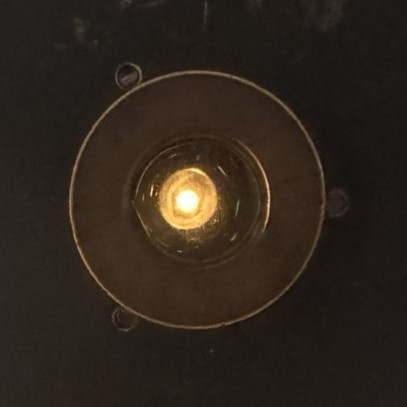
\includegraphics[width = 0.9\textwidth]{exp_pics/5_lam2_90}
        \caption{при скрещенных поляризациях}
    \end{subfigure}
    \hfill
    \begin{subfigure}{0.13\textwidth}
        \centering
        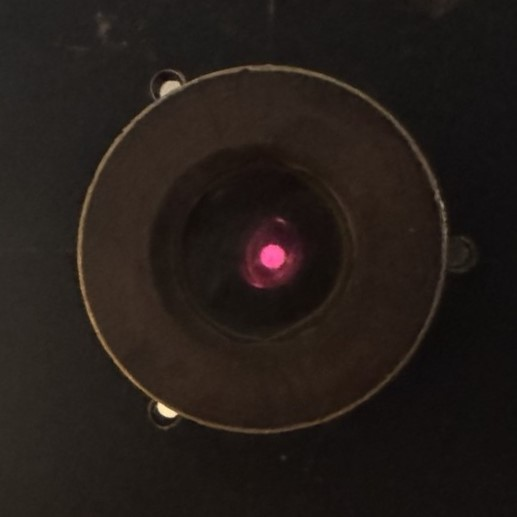
\includegraphics[width = 0.9\textwidth]{exp_pics/5_lam2_0}
        \caption{при параллельных поляризациях}
    \end{subfigure}
\end{wrapfigure}

Для различия пластинок $\frac{\lambda}{2}$ и $\frac{\lambda}{4}$ использовалась схема из предыдущего пункта. При этом главные оси исследуемой пластинки устанавливались под углом $45^\circ$ к разрешенному горизонтальному направлению первого поляроида, и наблюдалось изменение интенсивности при вращении второго поляроида.

Тогда после прохождения пластинки $\frac{\lambda}{4}$ (1), линейная поляризация, в соответствии с разделом \ref{subsec:polar_lam}, становилась круговой, поэтому при всех направлениях второго поляроида наблюдалась одинаковая интенсивность.

После прохождения же пластинки $\frac{\lambda}{2}$ (2), горизонтальная поляризация, в соответствии с разделом \ref{subsec:polar_lam}, становилась вертикальной, поэтому максимум и минимум интенсивности наблюдались при параллельных и скрещенных поляризациях поляроидов соответственно (см. Рис. \ref{fig:5}).


\subsection{Определение <<быстрой>> и <<медленной>> осей пластинки $\frac{\lambda}{4}$ с помощью пластинки чувствительного оттенка}

\begin{wrapfigure}{r}{0.35\textwidth}
    \begin{center}
    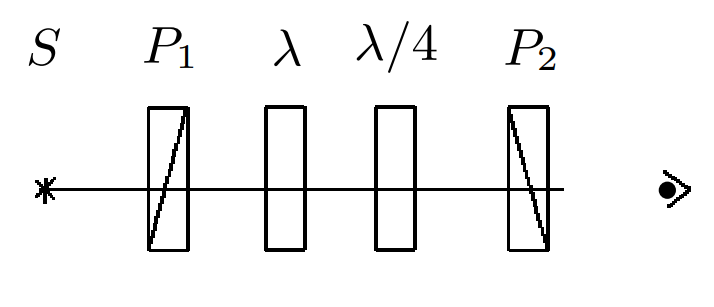
\includegraphics[width = 0.25\textwidth]{pics/setup_6}
    \caption{Определение направлений
большей и меньшей скорости}
    \label{fig:setup_6}
    \end{center}
\end{wrapfigure}

Для определения <<быстрой>> и <<медленной>> осей пластинки $\frac{\lambda}{4}$, была собрана схема \ref{fig:setup_6}. Пластинка чувствительного оттенка была размещена под углом $45^\circ$ между скрещенными поляроидами (см. Рис. \ref{fig:lam_90}). За ней располагалась исследуемая пластинка $\frac{\lambda}{4}$, главные оси которой последовательно соединялись с <<быстрой>> осью пластинки чувствительного оттенка. Таким образом, в согласии с разделом \ref{subsec:color_pl} была определена <<быстрая>> главная ось нашей пластинки $\frac{\lambda}{4}$ -- $148^\circ \leftrightarrow 328^\circ$ (см. Рис. \ref{fig:lam54_90} и \ref{fig:lam34_90}).

\begin{figure}[h]
    \caption{Пластинка чувствительного оттенка между скрещенных поляроидов}
    \centering
  \begin{subfigure}[t]{0.3\textwidth}
    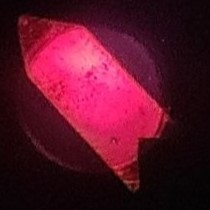
\includegraphics[width=0.9\textwidth]{exp_pics/6_lam_90}
    \caption{без $\frac{\lambda}{4}$}
    \label{fig:lam_90}
  \end{subfigure}
  \hfill
\begin{subfigure}[t]{0.3\textwidth}
    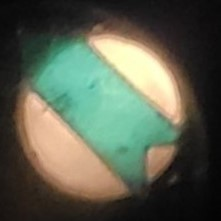
\includegraphics[width=0.9\textwidth]{exp_pics/6_lam54_90}
    \caption{с $\frac{\lambda}{4}$, <<быстрые>> оси совпадают}
    \label{fig:lam54_90}
  \end{subfigure}
  \hfill
  \begin{subfigure}[t]{0.3\textwidth}
    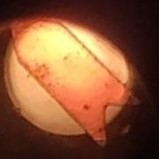
\includegraphics[width=0.9\textwidth]{exp_pics/6_lam34_90}
    \caption{с $\frac{\lambda}{4}$, <<быстрая>> и <<медленная>> оси совпадают}
    \label{fig:lam34_90}
  \end{subfigure}
\end{figure}



\subsection{Наблюдение интерференции поляризованных лучей на примере мозаичной слюдяной пластинки}

Для наблюдения эффектов, описанных в разделе \ref{subsec:polariz}, использовалась мозаичная слюдяная пластинка, собрана из 4-х узких полосок слюды, лежащих по сторонам квадрата: две полоски «толщиной» $\frac{\lambda}{4}$, и по одной $\frac{\lambda}{2}$, $\frac{3\lambda}{4}$ (см. Рис. \ref{fig:7_loc}).

\begin{figure}[h]
    \centering
  \begin{subfigure}[t]{0.24\textwidth}
    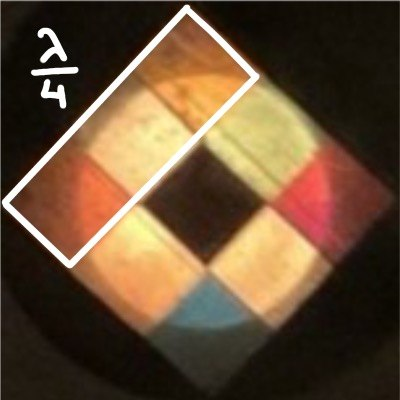
\includegraphics[width=0.9\textwidth]{exp_pics/7_loc_1}
  \end{subfigure}
  \hfill
\begin{subfigure}[t]{0.24\textwidth}
    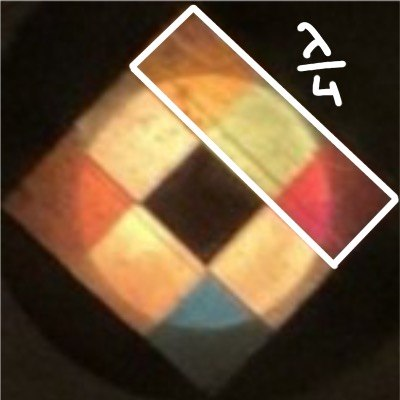
\includegraphics[width=0.9\textwidth]{exp_pics/7_loc_2}
  \end{subfigure}
  \hfill
\begin{subfigure}[t]{0.24\textwidth}
    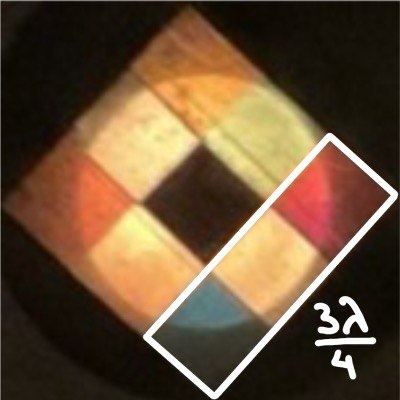
\includegraphics[width=0.9\textwidth]{exp_pics/7_loc_3}
  \end{subfigure}
  \hfill
\begin{subfigure}[t]{0.24\textwidth}
    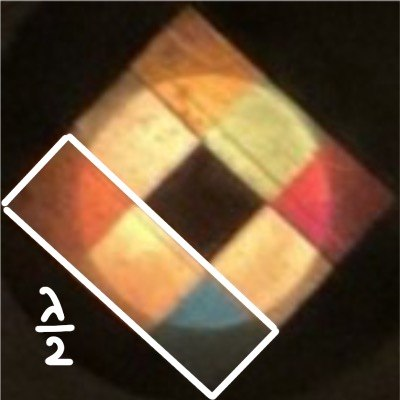
\includegraphics[width=0.9\textwidth]{exp_pics/7_loc_4}
  \end{subfigure}
  \caption{Расположение двоякопреломляющих пластинок в слюдяной мозаике}
    \label{fig:7_loc}
\end{figure}

Повотот пластинки при скрещенных поляроидах не менял цветов мозаики, но менял их яркость: когда главные оси пластинки совпадали с осями поляроидов, она не пропускала свет.

Поворот же второго поляроида при фиксированном положении пластинки, приводил к изменению цвета: как и ожидалось, при изменении положения поляроидов от скрещенного к параллельному, цвета мозаики изменялись на дополнительные (см. Рис. \ref{fig:7})

\begin{figure}[h]
    \centering
    \caption{Изменение цвета пластинки при разных углах между поляроидами}
    \label{fig:7}
  \begin{subfigure}[t]{0.3\textwidth}
    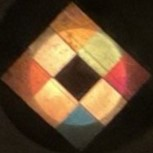
\includegraphics[width=0.9\textwidth]{exp_pics/7_90}
    \caption{$\beta = 90^\circ$}
  \end{subfigure}
  \hfill
\begin{subfigure}[t]{0.3\textwidth}
    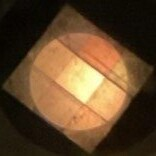
\includegraphics[width=0.9\textwidth]{exp_pics/7_45.png}
    \caption{$\beta = 45^\circ$}
  \end{subfigure}
  \hfill
\begin{subfigure}[t]{0.3\textwidth}
    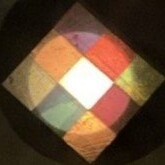
\includegraphics[width=0.9\textwidth]{exp_pics/7_0.png}
    \caption{$\beta = 0^\circ$}
  \end{subfigure}
\end{figure}

\subsection{Определение направления вращения эллиптически-поляризованного света с помощью пластинки $\frac{\lambda}{4}$}

Для <<генерации>> эллиптически поляризованного света использовалась пластинка $\frac{\lambda}{4}$ с соседней установки и поляризатор, установленный перед ней. Был получен эллиптически поляризованных свет с вертикальной малой полуосью. Установив на оптическую скамью изученную нами пластину $\frac{\lambda}{4}$ с горизонтальной <<быстрой>> полуосью, и проанализировав поляризацию на выходе вторым поляроидом, мы увидели, что итоговое направление линейной поляризации находится в I-III квадрантах. Согласно \ref{fig:ellipt_polar}, это значит, что изначально свет был поляризован по часовой стрелке.

\section{Заключение}

В первой части работы при помощи поляроидов, у которых предварительно были определены разрешенные направления, по углу Брюстера был определен коэффициент преломления эбонита, а также изучена поляризация отраженного и преломленного света.

Во второй части работы при помощи поляроидов и пластины чувствительного оттенка были определены главные оси двоякопреломляющих пластин, а также наблюдалась интерференция поляризованного света в мозаичной пластине. Далее с помощью изученной пластины $\frac{\lambda}{4}$ было определено направление вращения вектора напряженности в эллиптически поляризованном свете. 

Хотя работа носит скорее качественный и наблюдательный характер, полученные в ней результаты описываются теорией, которая четко предсказывает величину угла брюстера, поляризацию отраженного и преломленного света, хакартек интерференции поляризованных лучей и характер поляризации света при проходе двоякопреломляющих пластинок. 

\end{document}